%\documentclass{cumcmthesis}
\documentclass[withoutpreface,bwprint]{cumcmthesis} %去掉封面与编号页,电子版提交的时候使用。
\usepackage[superscript]{cite}
\usepackage{booktabs}
\usepackage{longtable}
\usepackage{float}
\usepackage{graphicx}
\usepackage{float}
\usepackage[framemethod=TikZ]{mdframed}
\usepackage{url}   % 网页链接
\usepackage{subcaption} % 子标题
\title{数学建模论文排版}
 
\begin{document}
\maketitle
\begin{abstract}

	这里写摘要,国赛论文摘要要求是一页最好,不要多也不要太少。

	%\keywords{ 科幻小说 \quad  摘要 \quad 三体  \quad  关键字 \quad 科学边界}
	\noindent{ \textbf{关键词:} Fisher精确检验\quad   多元线性回归\quad 系统聚类 \quad 灰色关联分析\quad}
\end{abstract}


\section{问题重述}
某电子产品的生产企业需要综合诸多考虑购置零部件、产品抽检、产品拆解、报废等问题,以确保产品质量的同时降低成本。

\textbf{问题一:}考虑到零配件供应商所述次品率不高于既定标称值,企业拟采用抽样检测方法以验收此批零配件。因为企业寻承担检测费用,企业希望应用数学模型得到最少抽检次数的抽样方案。

已知标称值为 10\%,结合以下两种不同情况,分别设计出具体的抽样检测方案:

1. 拒收条件:在95\%的置信水平下,如果检测结果表明零配件的次品率超出了标称值,那么这批零配件将被拒收。

2. 接收条件:在90\%的置信水平下,如果检测结果表明零配件的次品率未超过标称值,那么这批零配件将被接收。

\textbf{问题二:}在已知零配件及成品次品率情况下,在电子产品生产的零配件检测、装配、成品检测、不合格品拆解的各个阶段为企业作出最优决策。
并且结合判断依据及相应的指标对表1中企业在生产中遇到的情况作出相应的最优决策方案。

\textbf{问题三:}在零配件、半成品和成品的次品率已知情况下,重复问题2的生产决策方案以适配有m道工序、
n个零配件的问题。并且应用此方法针对表2中情况给出判断依据和指标得到最优的决策方案。

\textbf{问题四:}在零配件、半成品和成品的次品率均由抽样检测获得的情况下,重新考虑问题2、3的生产决策方案。
\section{问题分析}
\subsection{问题一的分析}
这里是第一段的内容。



\subsection{问题二的分析}
由于已知各零配件以及成品的次品率,依据排列组合我们能够得知在生产成品时零配件优劣的组合情况以及对应的概率分布。
又由于可能出现两个好的零部件组成一个坏的成品,综合成本考量我们需要考虑对成品拆解的比例。
我们预先设置对零配件、成品的抽样检测比例,通过多次模拟迭代实验得到最优的检测比例,以此来减少检测成本。
\subsection{问题三的分析}

\section{基本假设与符号说明}
\subsection{基本假设}
$\bullet$ 假设理论物理跟泵不存在;

$\bullet$ 假设数据中未填写的数据项为 0

$\bullet$ 假设所提供的数据准确无误;

$\bullet$ 不考虑因检验手段等原因对数据值的影响。

\subsection{符号说明}
\begin{table}[H]
	\centering
	\setlength{\tabcolsep}{20mm}%调整长度
	\begin{tabular}{cc}
		\toprule[1.5pt]
		\textbf{符号}& \textbf{含义} 	       \\  %textbf可以给文字加粗
		\midrule[1pt]
		$W_{j}$    & 基站${j}$的服务量         \\
		\bottomrule[1.5pt]
	\end{tabular}
\end{table}

\section{问题一模型的建立与求解}
针对每批零配件,假定总量为$N$,我们考虑采用异常检测的经典取样方法:序贯概率比检测$SPRT$作为抽检方案。在此之前
我们考虑每次取样的样本量为$D_i$,令单个零件次品与否的布尔值为$x$,考虑其单次试验成功(为次品)概率的期望为$\mu$,则其显然
服从经典的二项分布表示:
\begin{equation}
	\textit{Bern}(x|\mu) = \mu^x (1 - \mu)^{1-x}
\end{equation}
接下来考虑其在样本集上的对数似然函数,针对第$i$次取样$D_i$,对其中的每个样本取到观测$x_1,x_2...x_n$,根据题目要求
样本集中零配件的次品产生事件可认定为相互独立的。则其似然函数可写为:
\begin{equation}
	\mathbf{P}(D_i|\mu) = \prod_{n=1}^{N} p(x_n|\mu) = \prod_{n=1}^{N} \mu^{x_n} (1 - \mu)^{1-x_n}
\end{equation}
为便于后续处理,我们取其对数似然:
\begin{equation}
	\begin{split}
		&\ln\mathbf{P}(D|\mu) = \ln \prod_{n=1}^{N} \mu^{x_n} (1 - \mu)^{1-x_n}
		= \ln \mu \sum_{n=1}^{N} x_n + \ln(1 - \mu) \sum_{n=1}^{N} 1 - x_n \\
		&=  \ln \mu \sum_{n=1}^{N} x_n + \ln(1 - \mu) (N - \sum_{n=1}^{N} x_n)
		= \sum_{n=1}^{N} x_n \ln \mu + (1 - x_n) \ln(1 - \mu)
	\end{split}
\end{equation}
接下来我们依据题干给定零假设和备择假设:
\begin{equation}
	\begin{cases}
		H_0: \mu > 0.1 \\
		H_1: \mu \le 0.1
	\end{cases}
\end{equation}
题干中的两种情况意味着拒真和纳伪的显著性水平$\alpha$和$\beta$分别为0.05和0.1。在\textit{SPRT}语境下,考虑决策边界:
$$ A = \ln \frac{\beta}{1 - \alpha} \ \ \ \  B = \ln \frac{1 - \beta}{\alpha}$$
于是,针对每次采样$D_i$,我们需要求出在零假设和备择假设下的似然比$LR$:
\begin{equation}
	LR= \frac{\sum_{n=1}^{N} x_n \ln \mu_0 + (1 - x_n) \ln(1 - \mu_0)}{\sum_{n=1}^{N} x_n \ln \mu_1 + (1 - x_n) \ln(1 - \mu_1)}
\end{equation}
需要注意的是,在原生的$SPRT$场景中,$H_0$和$H_1$一般被认定为较为复杂的参数估计$\theta_0$和$\theta_1$,这取决于它们事先假定样本服从一个较为严谨且高度可表达的
概率分布。然而基于问题一,在没有明确历史数据和概率分布的先验情况下,我们只能将其建模为一般二项分布,
为了遵循$SPRT$的使用场景,我们将二项分布参数建模为$\mu_0=0.1+\Delta \mu$ , $\mu_1=0.1-\Delta \mu$。通过轻微扰动量来拟合样本的分布与所报标称值
的差异,扰动量的设置取决于样本量的大小,这点我们将在后续给出实验和说明。

尽管在许多场景中单样本取样策略以及被证明取得了很好的效果,但考虑到题干背景,我们依然选择样本集作为采样标准。遵循$SPRT$方法,给定总零配件量$N$,初次取样
$D_i$应为按照标称值所取的总样本配比,即$D_1=0.1N$,而后计算出当前样本下的对数似然比$LR_1$。序贯检验比方法遵循以下停止法则:
\begin{equation}
	\gamma = \inf \left\{ n | n \geq 1, LR_n \in (A, B) \right\}
\end{equation}
具体来说,若$LR_1 \le A$,接受$H_0$假设;若$LR_1 \ge B$,接受$H_1$假设,否则继续采样。初次采样的样本量为$D_1=0.1N$,假定每次
采样的次品数为$n_i$,则此后每次采样量依据以下法则确定:
\begin{equation}
	D_{i+1}=D_i-n_i
\end{equation}
检验的完整流程可以作出如下表示:





\section{问题二的模型建立与求解}
\begin{figure}[H]
	\centering
	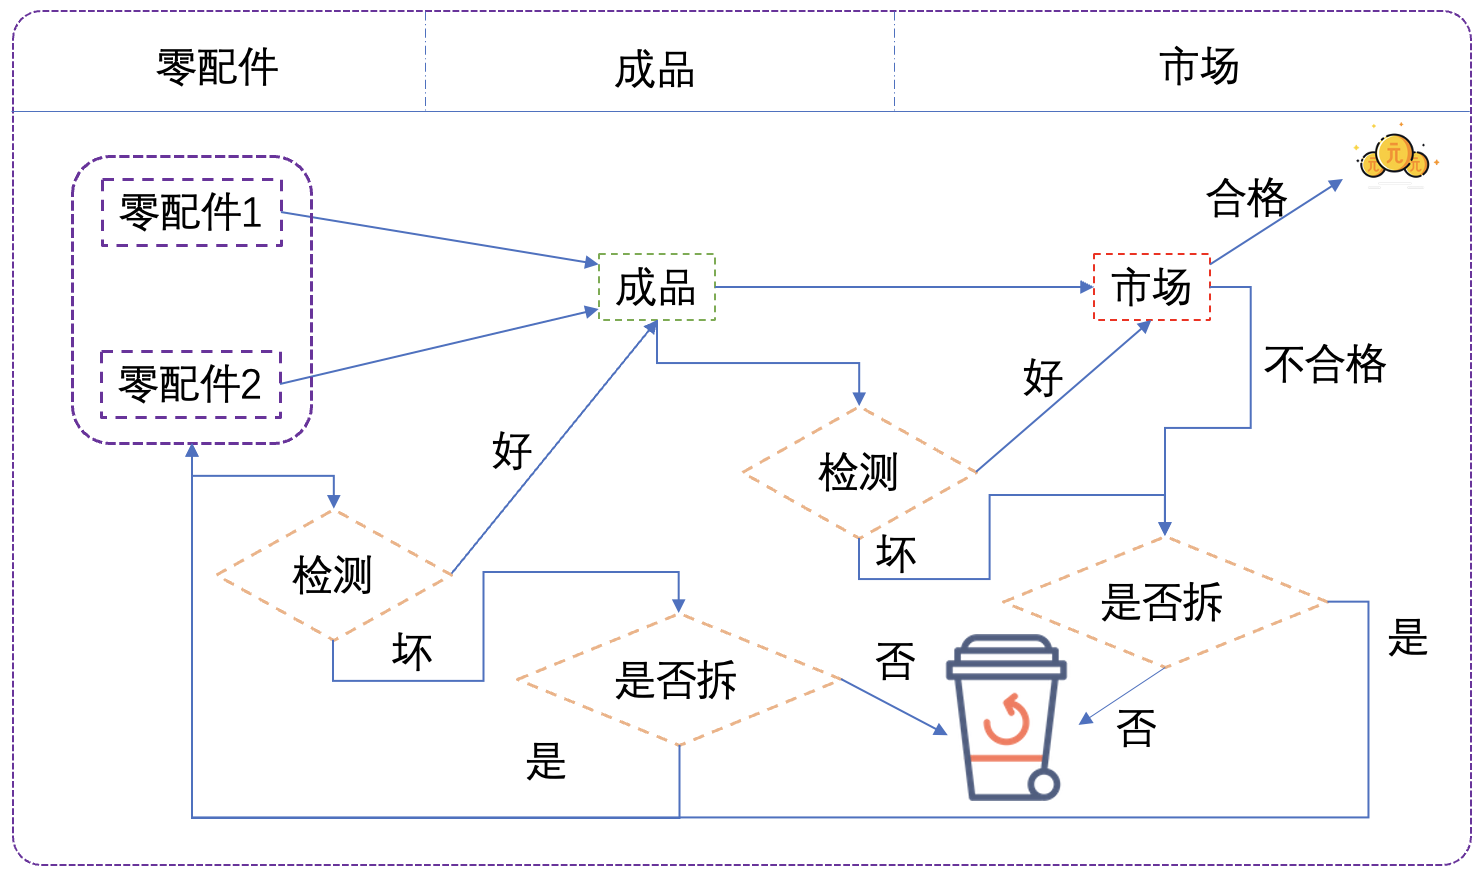
\includegraphics[width=0.6\textwidth]{pro2.png}      %获得的图片花括号中的名称为figure文件夹中重命名后的图片
	\caption{电子器件生产的流程图}
	\label{fig:pro2}
\end{figure}

\end{document}
